
In Section~\ref{prestudy}, we observe different patterns for the timing of proposing bounties, which may have different relationships with the issue-addressing likelihood. In this section, we investigate the relationship between the timing of proposing bounties and the issue-addressing likelihood. With a better understanding of the relationship, we can provide insights into how to improve the timing of proposing a bounty.

\textbf{Approach:}
We use the same data (100 samples of 1,500 issue reports for each sample) as RQ1. For each sample, we grouped data into four timing ranges based on the number of elapsed days between the creation of an issue report and the proposal of its first bounty(i.e., \textit{days-before-bounty}). We defined the four timing ranges as follows:
\begin{enumerate}
    \item \textbf{[0,7]:} the first bounty was proposed within seven days after the issue was reported.
    \item \textbf{(7,30]:} the first bounty was proposed between 7 and 30 days after the issue was reported.
    \item \textbf{(30,180]:} the first bounty was proposed between 30 and 180 days after the issue was reported.
    \item \textbf{(180,$\infty$):} the first bounty was proposed after 180 days after the issue was reported.
\end{enumerate}

Then we calculate the issue-addressing likelihood across the timing ranges for each sample to study the relationship between the timing and issue-addressing likelihood.
To further study the relationship between the issue-addressing speed and the timing, we also calculate the time it takes to close the issue report after the first bounty is proposed (i.e., \textit{time-to-close}) in each timing range for each sample.
Furthermore, we also study the timing in terms of different project groups for each sample.
\begin{comment}
	
\begin{figure}[t]
\centering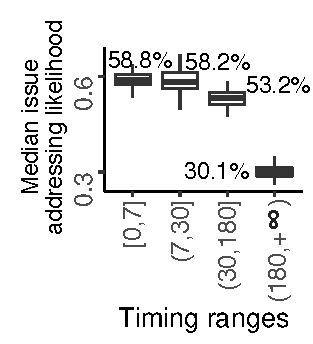
\includegraphics[width=\columnwidth]{pics/rq2/new/rq2_delta_ratio}
  \caption{The distribution of the median issue-addressing likelihood across the  timing ranges for the 100 studied samples.}
  \label{fig:rq2_delta_ratio}
  \vspace{-0.1in}

\end{figure}
\begin{figure}[t]
\centering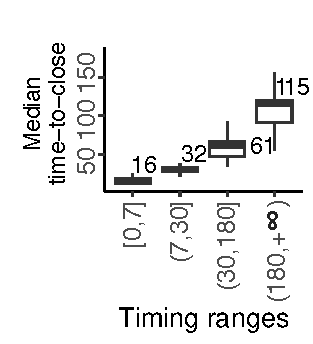
\includegraphics[width=\columnwidth]{pics/rq2/new/rq2_closeday_deltaday}
  \caption{The distribution of the median time to close an issue report (i.e., \textit{time-to-close}) for each timing range for 100 samples.}
  \label{fig:rq2_closeday_deltaday}
  \vspace{-0.1in}
\end{figure}
\end{comment}

\begin{figure}[t]
    \centering
    \begin{subfigure}[t]{0.5\columnwidth }
        \centering
        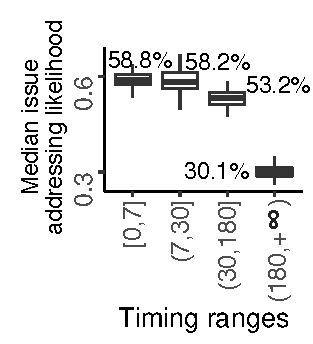
\includegraphics[width=\linewidth]{pics/rq2/new/rq2_delta_ratio}
        \caption{}
		\label{fig:rq2_delta_ratio}
    \end{subfigure}%
    ~
    \begin{subfigure}[t]{0.5\columnwidth}
        \centering
        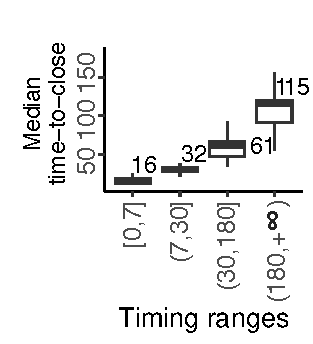
\includegraphics[width=\linewidth]{pics/rq2/new/rq2_closeday_deltaday}
        \caption{}
          \label{fig:rq2_closeday_deltaday}
    \end{subfigure}
    \vspace{-0.1in}
    \caption{The distribution of the median issue-addressing likelihood (a) and the  distribution of the median time to close an issue report (i.e., \textit{time-to-close}) (b) across the  timing ranges for the 100 studied samples.
    }
\end{figure}
\begin{figure}[t]
\centering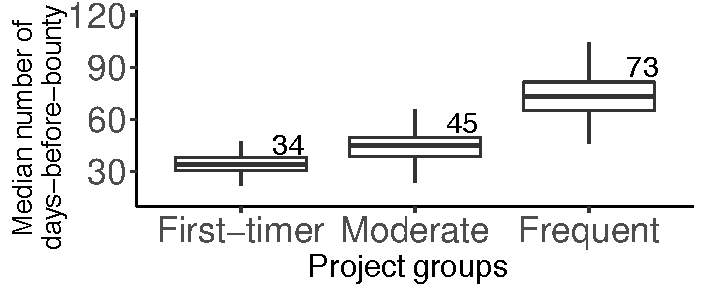
\includegraphics[width=0.8\columnwidth]{pics/rq2/new/rq2_medianDeltaTime.pdf}
  \caption{The distribution of the median number of days between the creation of the issue report and the proposed of the first bounty to the bounty is proposed (i.e., \textit{days-before-bounty}) across different project groups for 100 samples.}
  \label{fig:rq2_medianDeltaTime}
  \vspace{-0.15in}

\end{figure}




\noindent\textbf{Results:}\textbf{ In general, issue reports for which bounties were proposed earlier have a higher likelihood of being addressed.} Figure~\ref{fig:rq2_delta_ratio} shows the distribution of the median issue-addressing likelihood across the timing ranges over 100 samples. We calculated the Wilcoxon rank-sum test and Cliff's delta test to measure the differences between two distributions. The results show that there is no significant difference between the distributions of ``[0,7]'' and ``(7,30]'' while there exist significant differences with large effect sizes for the other two distributions.
The likelihood is getting smaller as the \textit{days-before-bounty} gets larger, especially for the issue reports in which bounties are proposed after 180 days where the likelihood drops to 30\%.

One possible explanation is that as time progresses, the risk of a report becoming obsolete exists, leaving the issue report unaddressed even after a bounty is proposed.
For example, an issue report\footnote{\url{https://github.com/bhdouglass/uappexplorer/issues/69}} that was created on Feb 4, 2016 in the \code{uappexplorer} project requested a new feature for an Ubuntu Phone Application.
The owner of the application and another developer both showed great interest in this issue. Because of the lack of time, the feature was never added. A bounty of \$5 was proposed\footnote{\url{%https://www.bountysource.com/issues/30521886-allow-comments-on-wishlist-items/backers
http://bit.ly/2Q3BIns}} after almost one year (i.e., on Jan 12, 2017).
However, the issue report was closed because Ubuntu Phone was no longer used making the issue report obsolete. Because of the low value, the bounty was not refundable. In other words,\textbf{ backers carry the risk of wasting their money by proposing small bounties on such long-standing issue reports.}

Another possible reason for the lower issue-addressing likelihood of the issue reports for which bounties were proposed later is the potential difficulty of such issue reports.
Figure~\ref{fig:rq2_closeday_deltaday} shows the median time that was taken to close issues (i.e., \textit{time-to-close}) across each timing range. We observe that the issue reports in which bounties were proposed later took more time to be addressed.




\textbf{Backers proposed bounties earlier in the first-timer bounty-projects.}
Figure~\ref{fig:rq2_medianDeltaTime} presents the distribution of the median value of the \textit{days-before-bounty} metric across the project groups for each sample. The median \textit{days-before-bounty} is 34, 45 and 73 for each project group, respectively.
We calculated the Wilcoxon rank-sum test and Cliff's delta $d$ effect size to measure the differences of distributions between the first-timer bounty-projects and the moderate bounty-projects, the moderate bounty-projects and the frequent bounty-projects, respectively. The result shows that any two pairs of distributions are significantly different with large Cliff's delta effect sizes, indicating that the \textit{days-before-bounty} is higher in projects with a higher bounty-usage frequency.
One explanation is that the activity of first-timer bounty-project is lower (see Figure~\ref{fig:rq1_activity}), which may encourage backers to propose a bounty earlier to attract developers to get an issue addressed.

%For example, Figure~\ref{fig:rq1_activity} shows that the first-timer projects have the smallest number of forks among all three project groups.



\rqbox{In general, issue reports for which bounties were proposed earlier have a higher likelihood of being addressed. In addition, the risk of losing money exists for backers who propose small bounties for long-standing issue reports.
}

